% Reviewed translation: PDF pages 146--152 / printed pages 132--138.
% The original scan is authoritative; environment headings remain English.
\MathBookSourcePage{146}
\section{采用不连续压力的单纯形有限元方法}
\label{sec:primitive-simplicial-discontinuous-pressure}

本节讨论的方法实质上是为求解 Stokes 和 Navier--Stokes 问题而发展出的
最早一批有限元方法. 自 Fortin [29] 以及 Crouzeix \& Raviart [23]
首次发表这些方法以来, 许多作者对它们作了实质性的简化和推广.
这里将研究 Bernardi \& Raugel [10], Fortin [30], Johnson \&
Pitk\"aranta [46], Mansfield [56] 以及 Boland \& Nicolaides [12]
的工作. 情形和记号与 Subsection~\ref{subsec:primitive-homogeneous-stokes}
相同.

\MathBookSourcePage{147}
\subsection{三角形单元上的一阶逼近}
\label{subsec:primitive-triangle-first-order}

本小节始终假设 $\Omega$ 是 $\mathbb{R}^2$ 中的一个有界多边形,
因而可以完全三角剖分. 对每个 $h>0$, $\mathcal{T}_h$ 是由直径不超过
$h$ 的三角形 $\kappa$ 组成的 $\Omega$ 的一个三角剖分:
\[
\bar\Omega=\bigcup_{\kappa\in\mathcal{T}_h}\kappa.
\]

读者此时已经清楚, 相容空间 $X_h$ 和 $M_h$ 的选择, 无论其精度如何,
对于逼近的成功都至关重要. 例如, 最直接的一阶空间选择为
\[
\begin{aligned}
W_h&=\{\,w\in\mathcal{C}^0(\bar\Omega)^2;
       \ w|_\kappa\in P_1^2\quad\forall\kappa\in\mathcal{T}_h\,\},\\
X_h&=W_h\cap H_0^1(\Omega)^2,\\
Q_h&=\{\,q\in L^2(\Omega);
       \ q|_\kappa\in P_0\quad\forall\kappa\in\mathcal{T}_h\,\},\\
M_h&=Q_h\cap L_0^2(\Omega).
\end{aligned}
\]
但这种选择往往导致 $V_h=\{0\}$, Figure~\ref{fig:primitive-incompatible-pair}
中的简单例子便可验证这一点. 在那里, $X_h$ 只有两个自由度,
而 $V_h$ 的定义要求五个独立条件. 因此 $V_h=\{0\}$.

\begin{figure}[htbp]
\centering
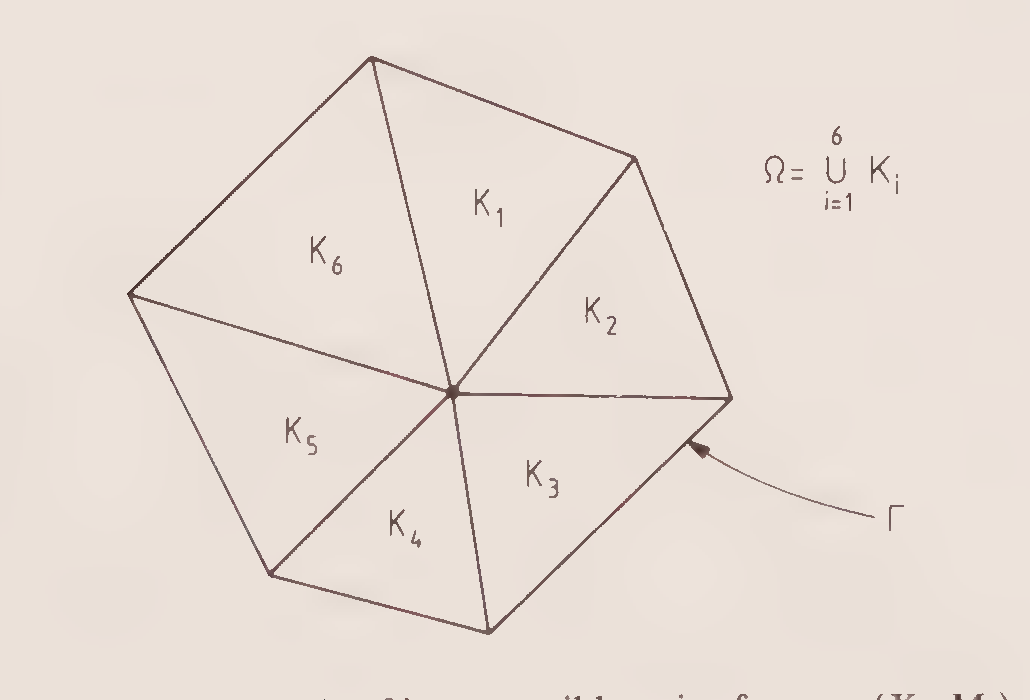
\includegraphics[width=.70\linewidth]{figures/chapter-02-figure-7.png}
\caption{不相容空间对 $(X_h,M_h)$ 的例子.}
\label{fig:primitive-incompatible-pair}
\end{figure}

这个例子说明, 为了生成足够大的空间 $V_h$, 空间 $W_h$ 需要更多自由度.
Fortin [29] 最初建议对 $W_h$ 中的函数采用分片二次多项式.

\MathBookSourcePage{148}
在很长一段时间里, 人们认为这是与上述压力空间 $Q_h$ 配合的最简单速度空间.
不过, 沿用 Fortin [30] 的另一个思路, Bernardi \& Raugel [10]
近来分析了一个中间速度空间, 它所需自由度较少, 也更容易推广到高阶情形.
下面详细研究这个单元.

设 $\kappa$ 是 $\mathcal{T}_h$ 的任意三角形, 其顶点如
Figure~\ref{fig:primitive-triangle-geometry} 所示为 $a_1,a_2,a_3$.
用 $f_i$ 表示与 $a_i$ 相对的边, 用 $\mathbf n_i$ 和 $\mathbf t_i$
分别表示 $f_i$ 上的单位外法向量和单位切向量. 我们要构造一个函数
$\mathbf w$, 它在 $\kappa$ 中的分量为二次多项式, 并且在每条边
$f_i$ 上的切向分量为仿射函数:
\[
\mathbf w|_\kappa\in P_2^2,
\qquad
\mathbf w\cdot\mathbf t_i|_{f_i}\in P_1.
\]
这可通过分解
\[
\mathbf w=\mathbf w_1+\mathbf w_2
\]
实现, 其中 $\mathbf w_1\in P_1^2$, $\mathbf w_2\in P_2^2$, 且
$\mathbf w_2\cdot\mathbf t_i|_{f_i}=0$.

\begin{figure}[htbp]
\centering
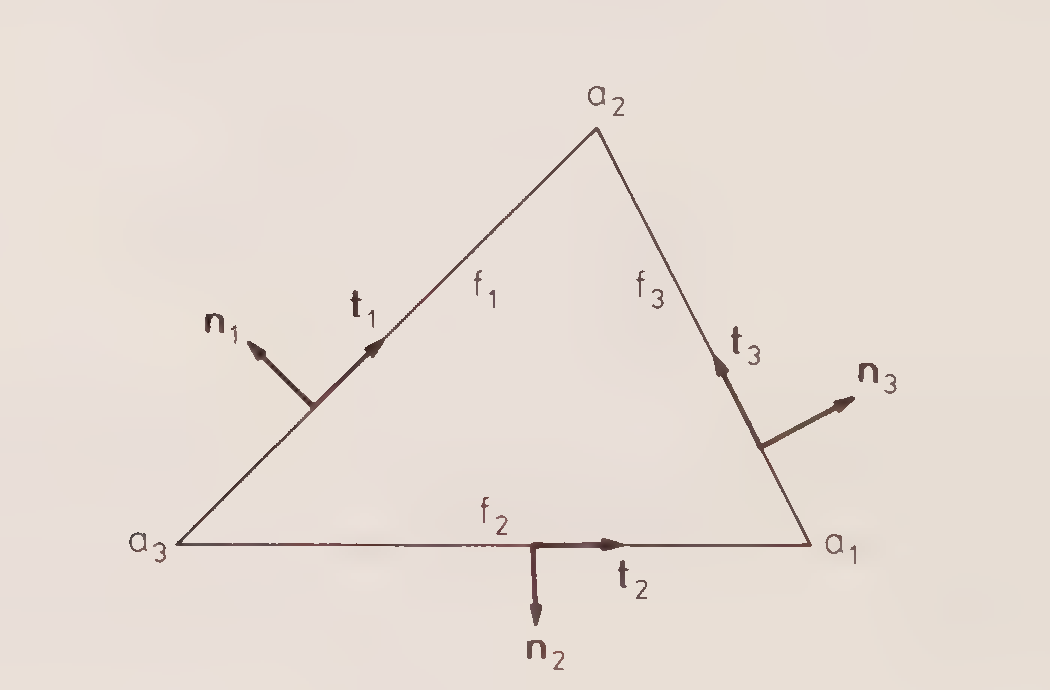
\includegraphics[width=.62\linewidth]{figures/chapter-02-figure-8.png}
\caption{三角形 $\kappa$ 的边、顶点、单位外法向量和单位切向量.}
\label{fig:primitive-triangle-geometry}
\end{figure}

例如, 注意函数
\[
\mathbf p_1=\mathbf n_1\lambda_2\lambda_3
\]
在边 $f_2$ 和 $f_3$ 上消失, 并满足
$\mathbf p_1\cdot\mathbf t_1|_{f_1}=0$. 推广这一观察, 置
\begin{equation}\label{eq:primitive-bernardi-raugel-bubbles}
\mathbf p_1=\mathbf n_1\lambda_2\lambda_3,
\qquad
\mathbf p_2=\mathbf n_2\lambda_3\lambda_1,
\qquad
\mathbf p_3=\mathbf n_3\lambda_1\lambda_2,
\end{equation}
并在 $P_2^2$ 的下列多项式子空间中选取速度 $\mathbf w$:
\begin{equation}\label{eq:primitive-bernardi-raugel-local-space}
\mathcal{P}_1(\kappa)
=P_1^2\oplus\operatorname{span}\{\mathbf p_1,\mathbf p_2,\mathbf p_3\}.
\end{equation}
因此提出如下空间对:
\begin{equation}\label{eq:primitive-bernardi-raugel-velocity-spaces}
\left\{
\begin{aligned}
W_h&=\{\,\mathbf w\in\mathcal{C}^0(\bar\Omega)^2;
\ \mathbf w|_\kappa\in\mathcal{P}_1(\kappa)
\quad\forall\kappa\in\mathcal{T}_h\,\},\\
\bar X_h&=W_h\cap H_0^1(\Omega)^2.
\end{aligned}
\right.
\end{equation}

\MathBookSourcePage{149}
\begin{equation}\label{eq:primitive-bernardi-raugel-pressure-spaces}
\left\{
\begin{aligned}
Q_h&=\{\,q\in L^2(\Omega);
\ q|_\kappa\in P_0\quad\forall\kappa\in\mathcal{T}_h\,\},\\
\bar M_h&=Q_h\cap L_0^2(\Omega).
\end{aligned}
\right.
\end{equation}
(在 $\bar X_h$ 和 $\bar M_h$ 上方加横线是为了与
Subsection~\ref{subsec:primitive-discrete-inf-sup-methods} 的记号一致.)

\setcounter{statement}{0}
\begin{Remark}\label{rem:primitive-bernardi-raugel-decomposition}
设 $\mathbf p\in\mathcal{P}_1(\kappa)$, 并令
\[
I_\kappa\mathbf p=\sum_{i=1}^3\mathbf p(a_i)\lambda_i
\]
表示它在 $P_1^2$ 上的标准插值. 由于
$\mathbf p_i(a_j)=0$ 对 $1\leq i,j\leq3$ 成立, $\mathbf p$ 具有形式
\[
\mathbf p=I_\kappa\mathbf p+\sum_{i=1}^3\alpha_i\mathbf p_i,
\qquad \alpha_i\in\mathbb{R}.
\]
此外, 由于当 $i\ne j$ 时 $\mathbf p_i|_{f_j}=0$, 立即得到
\[
\alpha_i\mathbf p_i|_{f_i}
=(\mathbf p-I_\kappa\mathbf p)|_{f_i}.
\]
\end{Remark}

这个 Remark 表明, 对 $\mathcal{P}_1(\kappa)$ 中的函数 $\mathbf p$,
可以选择如下自由度: $\mathbf p$ 在 $\kappa$ 的顶点 $a_i$ 处的值,
以及 $\mathbf p$ 通过 $\kappa$ 每条边 $f_i$ 的通量. 下一个 Lemma
验证这些自由度对 $\mathcal{P}_1(\kappa)$ 的唯一可解性.

\setcounter{statement}{0}
\begin{Lemma}\label{lem:primitive-bernardi-raugel-unisolvence}
$\mathcal{P}_1(\kappa)$ 中的多项式 $\mathbf p$ 由下列量唯一确定:
\begin{equation}\label{eq:primitive-bernardi-raugel-dofs}
\left\{
\begin{aligned}
&\mathbf p(a_i),&&1\leq i\leq3,\\
&\int_{f_i}\mathbf p\cdot\mathbf n_i\,\mathrm ds,
&&1\leq i\leq3.
\end{aligned}
\right.
\end{equation}
此外, 在 $\kappa$ 的任意一条边 $f_i=[a_k,a_l]$ 上,
$\mathbf p$ 只依赖于定义在该边上的自由度, 即
$\mathbf p(a_k)$, $\mathbf p(a_l)$ 和
$\int_{f_i}\mathbf p\cdot\mathbf n_i\,\mathrm ds$.
\end{Lemma}

\begin{Proof}
首先注意, 
\eqref{eq:primitive-bernardi-raugel-dofs} 包含九个线性条件,
而 $\mathbf p$ 有九个系数. 因此只需证明: 若
\eqref{eq:primitive-bernardi-raugel-dofs} 中所有自由度均为零,
则 $\mathbf p=0$.

由 Remark~\ref{rem:primitive-bernardi-raugel-decomposition},
$I_\kappa\mathbf p=0$. 同样,
$\int_{f_i}\alpha_i\mathbf p_i\cdot\mathbf n_i\,\mathrm ds=0$, 即
\[
\int_{f_i}\alpha_i\lambda_j\lambda_k\,\mathrm ds=0.
\]
于是对 $1\leq i\leq3$ 有 $\alpha_i=0$, 从而 $\mathbf p=0$.
类似地, 若 $\mathbf p(a_k)=\mathbf p(a_l)=0$ 且
$\int_{f_i}\mathbf p\cdot\mathbf n_i\,\mathrm ds=0$,
则容易得到 $\mathbf p|_{f_i}=0$.
\end{Proof}

Lemma~\ref{lem:primitive-bernardi-raugel-unisolvence} 导出如下插值算子:
对 $\mathbf v\in\mathcal{C}^0(\bar\Omega)^2$, 令
$r_\kappa\mathbf v$ 为由下式定义的
$\mathcal{P}_1(\kappa)$ 中的唯一多项式:
\begin{equation}\label{eq:primitive-bernardi-raugel-local-interpolant}
\left\{
\begin{aligned}
r_\kappa\mathbf v(a_i)&=\mathbf v(a_i),&&1\leq i\leq3,\\
\int_{f_i}(r_\kappa\mathbf v-\mathbf v)\cdot\mathbf n_i\,\mathrm ds&=0,
&&1\leq i\leq3,
\end{aligned}
\right.
\end{equation}

\MathBookSourcePage{150}
并令
\[
r_h\mathbf v|_\kappa=r_\kappa\mathbf v
\qquad\forall\kappa\in\mathcal{T}_h.
\]
由 Lemma~\ref{lem:primitive-bernardi-raugel-unisolvence} 得
\[
r_h\in
\mathcal{L}(\mathcal{C}^0(\bar\Omega)^2;W_h)
\cap
\mathcal{L}((\mathcal{C}^0(\bar\Omega)\cap H_0^1(\Omega))^2;\bar X_h).
\]

但是, 若要验证 inf-sup 条件, 即 Hypothesis H3, 根据
Lemma~\ref{lem:primitive-fortin-criterion}, 直接使用适当的算子 $\pi_h$
更为方便. 乍看之下, 上面的算子 $r_h$ 似乎可行, 因为
\[
\int_\kappa\operatorname{div}(\mathbf v-r_\kappa\mathbf v)\,\mathrm dx
=\sum_{i=1}^3\int_{f_i}(\mathbf v-r_\kappa\mathbf v)
\cdot\mathbf n_i\,\mathrm ds=0.
\]
但严格说来, $r_h$ 并不满足 H3, 因为它定义在 $H^2(\Omega)^2$ 上,
而不是 $H^1(\Omega)^2$ 上. 因此必须用另一个不涉及 $\mathbf v$
在 $\kappa$ 的顶点处取值的算子替代 $r_h$. 解决这一困难最容易的方法,
是以 $\mathbf v$ 在 $X_h$ 上的投影 $P_h\mathbf v$ 的值替代
$\mathbf v$ 的值. 从实际观点看, 这种全局正则化并不令人满意,
因为相应证明要求三角剖分一致正则(参见 Theorem~\ref{lem:appendix-lagrange-interpolation}
以及 Girault \& Raviart [32]). 这一附加要求源于全局正则化,
而非上述逼近本身; 改用 Section~\ref{sec:appendix-interpolation-discontinuous-functions}
中的局部正则化算子即可去掉它.

因此, 按照 Bernardi \& Raugel [10], 对每个
$\mathbf v\in H_0^1(\Omega)^2$, 令 $\mathbf w_h=R_h\mathbf v\in\Phi_h^2$,
其中
\[
\Phi_h=\{\,\phi\in\mathcal{C}^0(\bar\Omega);
\ \phi|_\kappa\in P_1\quad\forall\kappa\in\mathcal{T}_h\,\}
\cap H_0^1(\Omega),
\]
且 $R_h$ 由 
\eqref{eq:appendix-local-regularization-projection} 和
\eqref{eq:appendix-local-regularization-interpolant} 定义. 然后定义算子
$\pi_h\in\mathcal{L}(H_0^1(\Omega)^2;\bar X_h)$:
\begin{equation}\label{eq:primitive-bernardi-raugel-fortin-operator}
\left\{
\begin{aligned}
\pi_h\mathbf v(a)&=R_h\mathbf v(a)
&&\forall\text{ $\mathcal{T}_h$ 的节点 }a,\\
\int_f(\pi_h\mathbf v-\mathbf v)\cdot\mathbf n\,\mathrm ds&=0
&&\forall\text{ $\mathcal{T}_h$ 的边 }f.
\end{aligned}
\right.
\end{equation}

现在假设三角剖分族 $\mathcal{T}_h$ 在
Definition~\ref{def:appendix-regular-triangulation} 的意义下正则, 即
\begin{equation}\label{eq:primitive-triangulation-regularity}
h_\kappa/\rho_\kappa\leq\sigma
\qquad\forall\kappa\in\mathcal{T}_h,
\qquad \sigma\text{ 与 }h\text{ 无关}.
\end{equation}
下面的 Lemma 表明 $\pi_h$ 满足 $l=1$ 时的 Hypothesis H1, 也满足
Hypothesis H3.

\setcounter{statement}{1}
\begin{Lemma}\label{lem:primitive-bernardi-raugel-fortin-estimates}
若三角剖分 $\mathcal{T}_h$ 正则, 则
\begin{equation}\label{eq:primitive-bernardi-raugel-interpolation-estimate}
|\mathbf v-\pi_h\mathbf v|_{m,\Omega}
\leq Ch^{k-m}|\mathbf v|_{k,\Omega}
\qquad\forall\mathbf v\in H^k(\Omega)^2,
\end{equation}
其中 $m=0$ 或 $1$, $k=1$ 或 $2$, 正常数 $C$ 与 $h$ 和
$\mathbf v$ 无关. 此外, 无论三角剖分是否正则, 都有
\begin{equation}\label{eq:primitive-bernardi-raugel-divergence-orthogonality}
\int_\Omega\operatorname{div}(\mathbf v-\pi_h\mathbf v)q\,\mathrm dx=0
\qquad\forall q\in Q_h.
\end{equation}
\end{Lemma}

\MathBookSourcePage{151}
\begin{Proof}
如上所述, \eqref{eq:primitive-bernardi-raugel-fortin-operator} 的第二式
直接给出 \eqref{eq:primitive-bernardi-raugel-divergence-orthogonality}.
取 $\mathcal{T}_h$ 的任意三角形 $\kappa$. 由
Remark~\ref{rem:primitive-bernardi-raugel-decomposition} 和
\eqref{eq:primitive-bernardi-raugel-fortin-operator} 的第一式得到
\[
\pi_h\mathbf v|_\kappa
=R_h\mathbf v|_\kappa+\sum_{i=1}^3\alpha_i\mathbf p_i,
\]
其中
\[
\alpha_i=
\left[\int_{f_i}(\mathbf v-R_h\mathbf v)\cdot\mathbf n_i\,\mathrm ds\right]
\left/\left[\int_{f_i}\lambda_j\lambda_k\,\mathrm ds\right]\right. .
\]
首先, 根据 Theorem~\ref{thm:appendix-local-regularization-error},
算子 $R_h$ 有如下局部插值误差:
\begin{equation}\label{eq:primitive-bernardi-raugel-local-regularization-error}
\|\mathbf v-R_h\mathbf v\|_{0,\kappa}
+h_\kappa|\mathbf v-R_h\mathbf v|_{1,\kappa}
\leq C_1h_\kappa^k|\mathbf v|_{k,\Delta_\kappa}
\qquad\forall\mathbf v\in H^k(\Omega)^2,
\end{equation}
其中 $k=1$ 或 $2$, $\Delta_\kappa$ 表示 $\mathcal{T}_h$ 中所有与
$\kappa$ 至少共用一个顶点的单元之并.

其次, 公式 \eqref{eq:appendix-gradient-transform} 给出
\begin{equation}\label{eq:primitive-bernardi-raugel-bubble-seminorm}
\left\{
\begin{aligned}
|\mathbf p_i|_{m,\kappa}
&\leq C_2|\det(B_\kappa)|^{1/2}
\|B_\kappa^{-1}\|^m
|\hat\lambda_j\hat\lambda_k|_{m,\hat\kappa}\\
&\leq C_3|\det(B_\kappa)|^{1/2}
\|B_\kappa^{-1}\|^m,
\end{aligned}
\right.
\end{equation}
因为 $|\hat\lambda_j\hat\lambda_k|_{m,\hat\kappa}$ 是与 $h$ 和
$\kappa$ 无关的常数. 类似地,
\[
\int_{f_i}\lambda_j\lambda_k\,\mathrm ds
=\frac{\operatorname{meas}(f_i)}{\operatorname{meas}(\hat f_i)}
\int_{\hat f_i}\hat\lambda_j\hat\lambda_k\,\mathrm d\hat s.
\]
最后,
\[
\left|\int_{f_i}(\mathbf v-R_h\mathbf v)\cdot\mathbf n_i\,\mathrm ds\right|
\leq\frac{\operatorname{meas}(f_i)}{\operatorname{meas}(\hat f_i)}
\int_{\hat f_i}|\hat{\mathbf v}-\widehat{R_h\mathbf v}|\,\mathrm d\hat s
\]
且由 trace Theorem~\ref{thm:trace-operator},
\[
\int_{\hat f_i}|\hat{\mathbf v}-\widehat{R_h\mathbf v}|\,\mathrm d\hat s
\leq C_4\|\hat{\mathbf v}-\widehat{R_h\mathbf v}\|_{1,\hat\kappa}.
\]
而由 \eqref{eq:appendix-gradient-transform} 和
\eqref{eq:appendix-simplex-matrix-bounds} 可得
\[
\|\hat{\mathbf v}-\widehat{R_h\mathbf v}\|_{1,\hat\kappa}
\leq C_5|\det(B_\kappa)|^{-1/2}
\left\{
\|\mathbf v-R_h\mathbf v\|_{0,\kappa}^2
+h_\kappa^2|\mathbf v-R_h\mathbf v|_{1,\kappa}^2
\right\}^{1/2}.
\]
因此 \eqref{eq:primitive-bernardi-raugel-local-regularization-error} 给出
\[
|\alpha_i|
\leq C_6|\det(B_\kappa)|^{-1/2}h_\kappa^k
|\mathbf v|_{k,\Delta_\kappa}.
\]
将它与 \eqref{eq:primitive-bernardi-raugel-bubble-seminorm},
\eqref{eq:appendix-simplex-matrix-bounds} 和
\eqref{eq:primitive-triangulation-regularity} 结合, 得到

\MathBookSourcePage{152}
\[
\left|\sum_{i=1}^3\alpha_i\mathbf p_i\right|_{m,\kappa}
\leq C_7\sigma^m h_\kappa^{k-m}|\mathbf v|_{k,\Delta_\kappa}.
\]
再应用一次 \eqref{eq:primitive-bernardi-raugel-local-regularization-error},
得到
\[
|\mathbf v-\pi_h\mathbf v|_{m,\kappa}
\leq C_8\sigma^m h^{k-m}|\mathbf v|_{k,\Delta_\kappa},
\qquad m=0,1,\quad k=1,2.
\]
而 $\mathcal{T}_h$ 的正则性意味着, 给定三角形 $\kappa$ 在各集合
$\Delta_\kappa$ 中出现的最大次数, 被一个与 $h$ 和 $\kappa$ 无关的
固定常数 $M$ 所控制. 因此
\[
\left(\sum_{\kappa\in\mathcal{T}_h}
|\mathbf v|_{k,\Delta_\kappa}^2\right)^{1/2}
\leq M|\mathbf v|_{k,\Omega},
\]
从而
\[
|\mathbf v-\pi_h\mathbf v|_{m,\Omega}
\leq C_8M\sigma^m h^{k-m}|\mathbf v|_{k,\Omega}.
\]
特别地, 当 $k=m=1$ 时, 这就建立了
Lemma~\ref{lem:primitive-fortin-criterion} 的界
\eqref{eq:primitive-fortin-stability}:
\[
|\pi_h\mathbf v|_{1,\Omega}
\leq(1+C_8M\sigma)|\mathbf v|_{1,\Omega}
\qquad\forall\mathbf v\in H_0^1(\Omega)^2.
\]
当 $k=2$, $m=1$ 时, 则得到 $l=1$ 的 Hypothesis H1.
\end{Proof}

最后, 对 $Q_h$ 上的 $L^2$ 投影 $\rho_h$, Hypothesis H2 直接由
Lemma~\ref{lem:appendix-local-l2-projection-error} 得出:
\begin{equation}\label{eq:primitive-bernardi-raugel-pressure-projection}
\|q-\rho_hq\|_{0,\Omega}
\leq Ch|q|_{1,\Omega}
\qquad\forall q\in H^1(\Omega).
\end{equation}
由于 Theorems~\ref{thm:primitive-homogeneous-stokes-convergence} 和
\ref{thm:primitive-stokes-l2-error} 的全部假设均满足,
便得到该一阶格式的如下收敛结果.

\setcounter{statement}{0}
\begin{Theorem}\label{thm:primitive-bernardi-raugel-convergence}
设 $\Omega$ 是有界平面多边形. 设 Stokes 问题的解
$(\mathbf u,p)$ 满足
\[
\mathbf u\in[H^2(\Omega)\cap H_0^1(\Omega)]^2,
\qquad
p\in H^1(\Omega)\cap L_0^2(\Omega),
\]
并分别由 \eqref{eq:primitive-bernardi-raugel-velocity-spaces} 和
\eqref{eq:primitive-bernardi-raugel-pressure-spaces} 定义空间
$\bar X_h$ 和 $\bar M_h$. 若三角剖分族 $\mathcal{T}_h$ 正则,
则 \eqref{eq:primitive-stokes-discrete-mixed} 的解
$(\mathbf u_h,p_h)$ 满足误差估计
\begin{equation}\label{eq:primitive-bernardi-raugel-h1-error}
|\mathbf u-\mathbf u_h|_{1,\Omega}
+\|p-p_h\|_{0,\Omega}
\leq C_1h(|\mathbf u|_{2,\Omega}+|p|_{1,\Omega}).
\end{equation}
此外, 若 $\Omega$ 为凸集, 则
\begin{equation}\label{eq:primitive-bernardi-raugel-l2-error}
\|\mathbf u-\mathbf u_h\|_{0,\Omega}
\leq C_2h^2(|\mathbf u|_{2,\Omega}+|p|_{1,\Omega}).
\end{equation}
\end{Theorem}

\setcounter{statement}{1}
\begin{Remark}\label{rem:primitive-bernardi-raugel-seminorm-estimates}
上述两个上界均以 $\mathbf u$ 和 $p$ 的半范数表示, 而
Theorems~\ref{thm:primitive-homogeneous-stokes-convergence} 和
\ref{thm:primitive-stokes-l2-error} 的估计右端包含全范数.
这一轻微改进源于 \eqref{eq:primitive-bernardi-raugel-local-regularization-error}
和 \eqref{eq:primitive-bernardi-raugel-pressure-projection} 都仅以半范数表述.
\end{Remark}
